\documentclass{beamer}
\usetheme{Warsaw}

\usepackage[utf8]{inputenc}
\usepackage{fancybox}
\usepackage{multimedia} 
\usepackage{subfig}
\usepackage{amsmath}

\usepackage[all]{xy}
\begin{document}


\title[Computergrafik] % (optional, only for long titles)
{Computergrafik}
\titlegraphic{%
    \begin{figure}[t]
        \centering
        \includegraphics[scale=0.26]{images/cover}
        \caption*{\scriptsize Quelle: https://iquilezles.org/}
    \end{figure}
}
\subtitle{}
\author[Dr. Johannes Riesterer] % (optional, for multiple authors)
{Dr.  rer. nat. Johannes Riesterer}

\date[KPT 2004] % (optional)
{}

\subject{Computergrafik}

\frame{\titlepage}

\begin{frame}
    \frametitle{Computergrafik}
\framesubtitle{}
    \begin{block}{Anwendungen}
\begin{itemize}
\item Interdisziplinär
\item Informatik
\item Technische Informatik
\item Mathematik
\item Physik
\item Psychologie
\item Ingenieurwissenschaften
\end{itemize}
\end{block}
\end{frame}

\begin{frame}
    \frametitle{Computergrafik}
\framesubtitle{}
    \begin{block}{Anwendungen}
\begin{itemize}
\item Simulation - virtuelle Realität 
\item Unterhaltung und Multimedia
\item Datenvisualisierung
\item Mensch-Maschine Interaktion - Assistenzsysteme - Augmented Reality
\item Industrie - CAD/CAM
\item Generative Gestaltung - KI
\end{itemize}
\end{block}
\end{frame}



\begin{frame}
\frametitle{Computergrafik}
\framesubtitle{Anwendungen}
 \begin{block}{Simulation - virtuelle Realität}
\includegraphics[scale=1.0]{images/Flugsimulator}
\includegraphics[scale=0.8]{images/Immersive_Simulation}
\end{block}
\end{frame}



\begin{frame}
\frametitle{Computergrafik}
\framesubtitle{Anwendungen}
 \begin{block}{Unterhaltung und Multimedia}
\begin{center}
\includegraphics[scale=1.0]{images/Pong}
\end{center}
\end{block}
\end{frame}



\begin{frame}
\frametitle{Computergrafik}
\framesubtitle{Anwendungen}
 \begin{block}{Datenvisualisierung}
\begin{center}
\includegraphics[scale=0.3]{images/Scatter_plot}
\end{center}
\end{block}
\end{frame}



\begin{frame}
\frametitle{Computergrafik}
\framesubtitle{Anwendungen}
 \begin{block}{Assistenzsystem - Augmented Reality}
\begin{center}
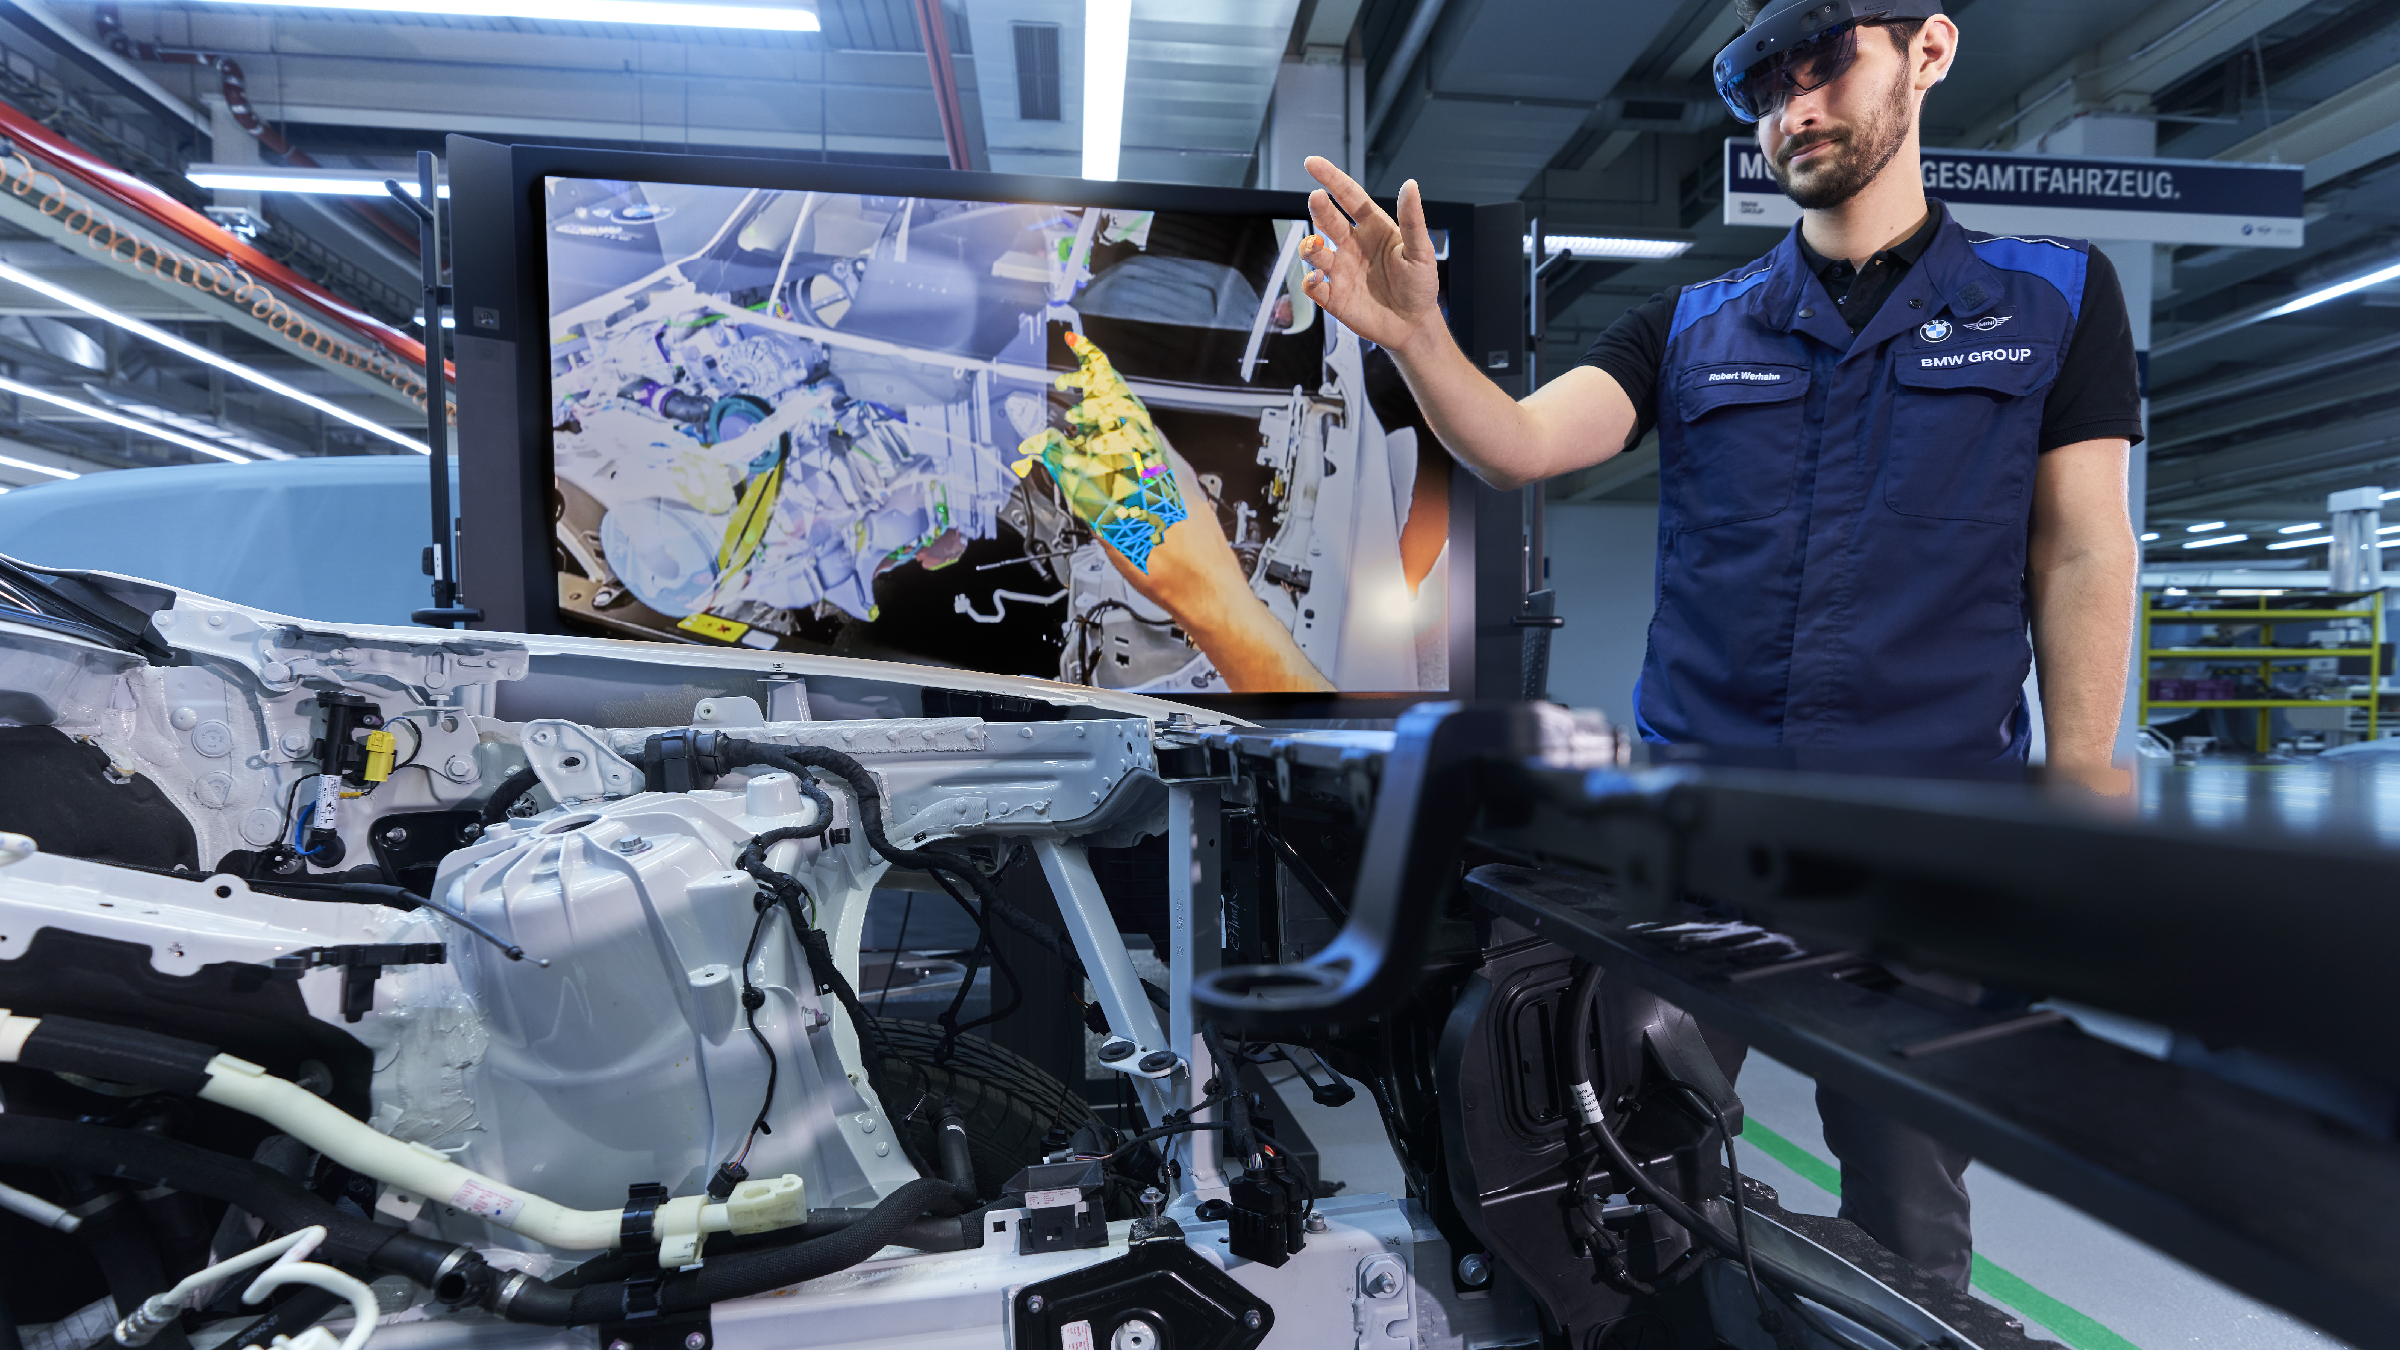
\includegraphics[scale=0.2]{images/Augmented}
\end{center}
\end{block}
\end{frame}



\begin{frame}
\frametitle{Computergrafik}
\framesubtitle{Anwendungen}
 \begin{block}{Mensch-Maschine Interaktion}
\begin{center}
\includegraphics[scale=0.55]{images/HCI}
\end{center}
\end{block}
\end{frame}


\begin{frame}
    \frametitle{Computergrafik}
\framesubtitle{}
    \begin{block}{Themen}
\begin{itemize}
\item Echtzeit Darstellung mit OpenGL
\item Mensch-Maschine Interaktion / User Experience
\item Physikalische Licht- und Farbmodelle. Gestaltungslehre
\item Generative KI 
\item Raytracing
\item Rechnerunterstütztes Konstruieren (CAD)
\item Mathematik/Physik
\end{itemize}
\end{block}

\end{frame}




\end{document}
